\bigskip
\begin{center}
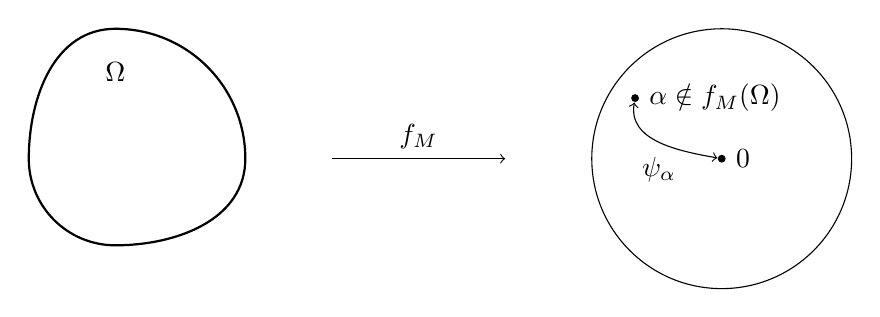
\begin{tikzpicture}[scale=1.1]
    \draw[thick] (0,0) to[out=90,in=180] (1,1.5) to[out=0,in=90] (2.5,0) 
    to[out=-90,in=0] (1,-1) to[out=180,in=-90] cycle;
    \node at (1,1) {$\Omega$};

    \draw [->] (3.5,0) -- (5.5,0) node [midway, above] {$f_M$};

    \draw[black] (8,0) circle (1.5);
    \node (alpha) [fill,circle,inner sep=1pt,label=right:$\alpha\notin f_M(\Omega)$] at (7,0.7) {};
    \node (origin) [fill,circle,inner sep=1pt,label=right:$0$] at (8,0) {};

    \draw[<->] (alpha) to[out=-100, in=170] node[below=2pt, pos=0.5] {$\psi_{\alpha}$} (origin);
\end{tikzpicture}
\end{center}
\bigskip